\chapter{UCNA Calibrations}
\label{ch:UCNA_Calibrations}
%%%%%%%%%%%%%%%%%%%%%%%%%%%%%%%%%%%%%%%%%%%%%%%%%%%%%%%%%%%%%%%%%%%%%%%%%%%%%%%
%%%%%%%%%%%%%%%%%%%%%%%%%%%%%%%%%%%%%%%%%%%%%%%%%%%%%%%%%%%%%%%%%%%%%%%%%%%%%%%
%%%%%%%%%%%%%%%%%%%%%%%%%%%%%%%%%%%%%%%%%%%%%%%%%%%%%%%%%%%%%%%%%%%%%%%%%%%%%%%

Detector calibrations are a beautiful combination
of simulation and data manipulation which allows one to extract the energy of
an event based solely on some electronic signal. Imagine a baseball pitcher
throwing a fastball into a sheet, and the observer behind the sheet must
determine the velocity of the ball from only seeing the impression the pitch
made on the sheet. This is the task every nuclear physics experiment is faced
with, only the baseball is a particle and the sheet is our detector system.
Below we focus on the energy calibration of our apparatus.

%--------------------------------------------------------------


%----------------------------------------------------------

\section{Wirechamber Calibration}

\subsection{Wirechamber signals}

The wirechamber signals for each detector include a summed anode signal, and two cathode signal
collections consisting of 16 individual ``wire'' readings. Again we use the term
wire loosely, as there are technically 64 wires in a plane, but they are read out in groups
of four. The position of each wire group is taken to be the midpoint of the grouping (between
the two center wires). The two sets of cathode signal collections come from perpendicular
planes, so the position can be reconstructed along both the $x-$ and $y-$axis.

The signal is read out by a peak sensing ADC, and so the maximum value of the signal is recorded
for each event. The pedestal is determined using the bismuth pulser events (different from the
PMT pedestals) and is subtracted from the ADC signal for every event. For the cathodes, a software
threshold for each wire is set at 100~channels above pedestal, so only wires above this threshold
will be used in the position reconstruction.

\subsubsection{Wirechamber trigger} \label{sssec:mwpctrigg}

As mentioned in sections \ref{sec:ExpMWPC} and \ref{sec:backscattering}, a wirechamber
software trigger is set and used to eliminate the gamma background and to identify different
backscattering events. One could use either the summed anode signal or a signal formed from
the cathode signals. The best trigger is one that separates the pedestal furthest from the
triggering data. For this analysis, this was found to be the sum of the maximum cathode
signals from the two wire planes. (Add figure of the two signals?)

\subsubsection{Cathode wire clipping}

Low energy event deposit a substantial amount of energy in the MWPC, and thus create large
signals in one or more wires in cathode planes. This can create a signal which is beyond the
range of the ADC, thus creating an overflow event which is read out as the max value of the ADC.
These events are called ``clipped'' events. A plot of the typical ratio of clipped events and the
number of clipped wires can be seen in figure \ref{fig:nClipped}.

\begin{figure}[h]
  \centering
  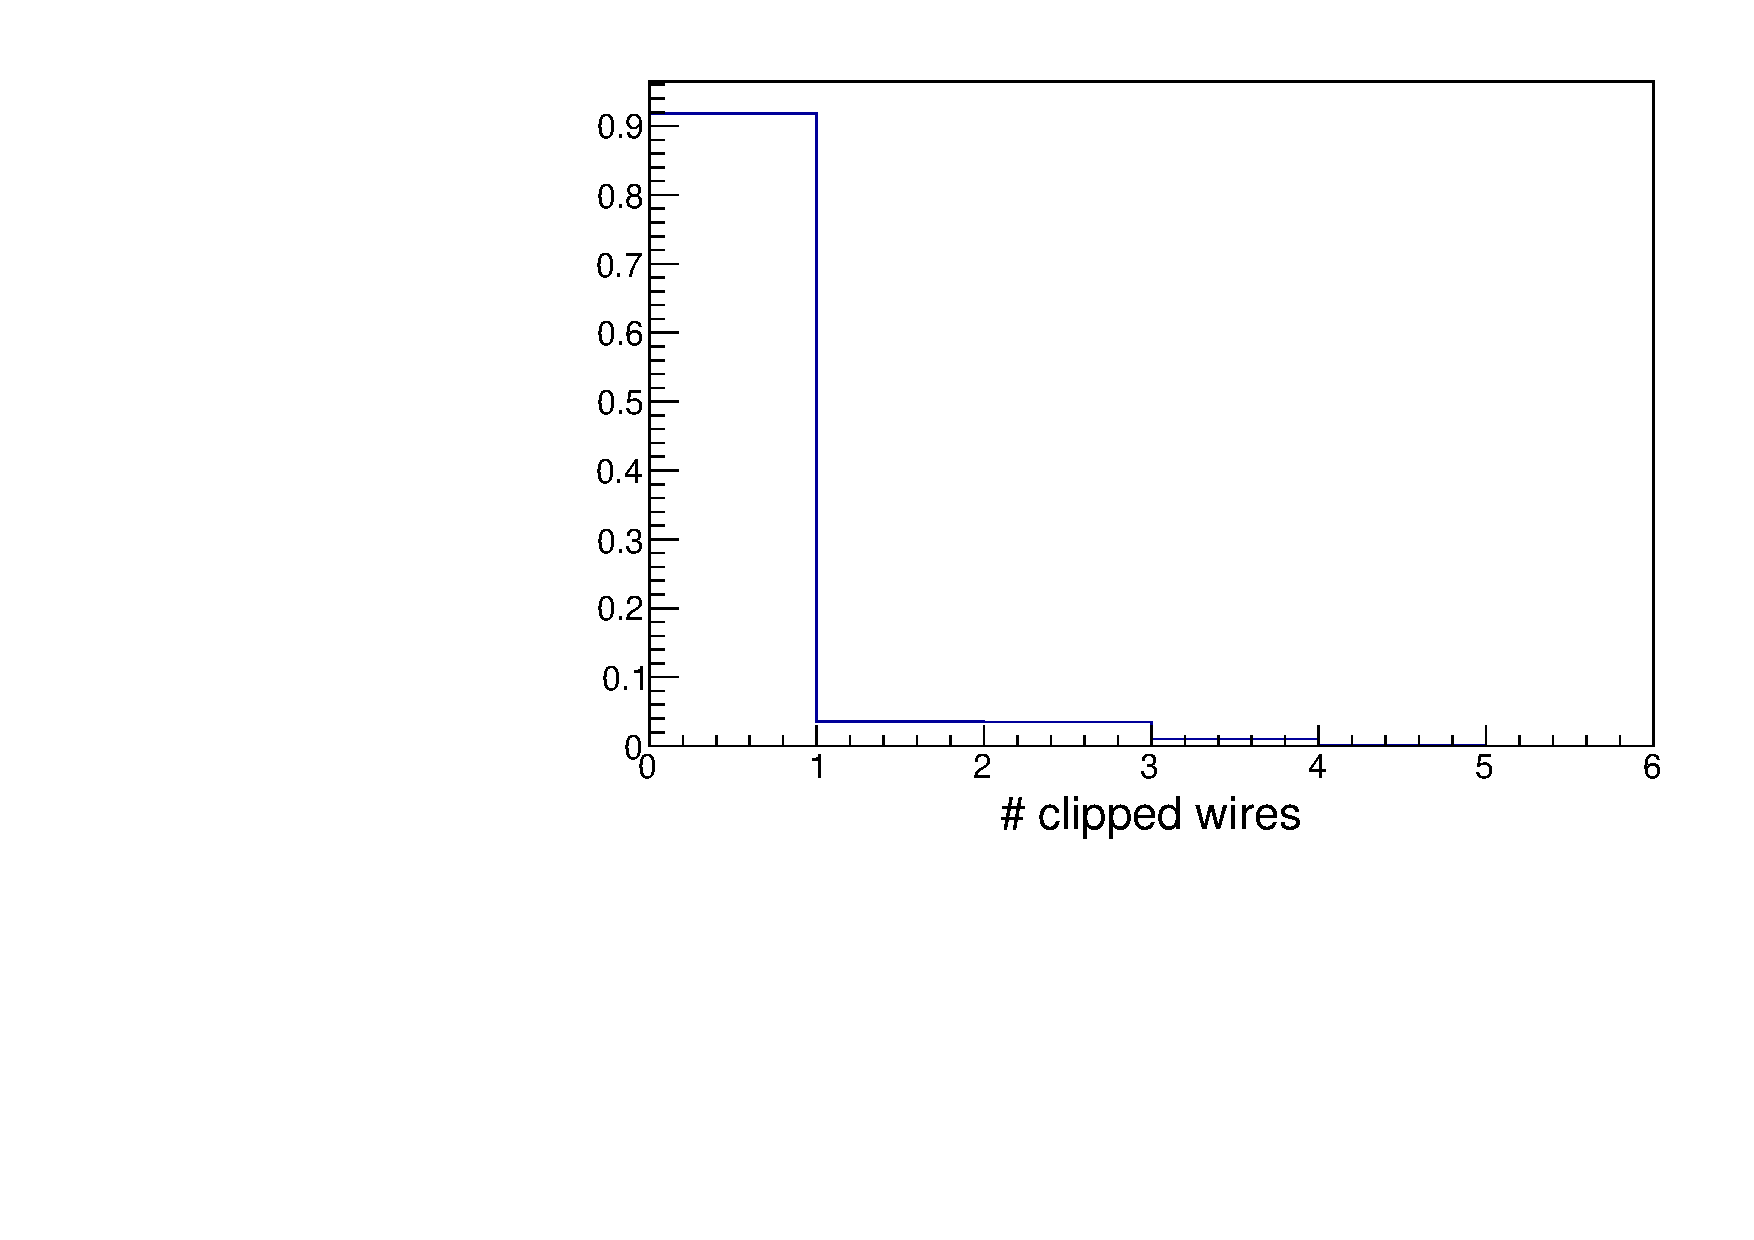
\includegraphics[scale=0.6,page=1]{4-UCNACalibrations/mwpc_position.pdf} 
  \caption{Number of clipped wires in the x-plane of the East detector. Most of the events
    (\~92~\%) exhibit no clipping.}
  \label{fig:nClipped}
\end{figure}


A clipped event poses a problem in the position reconstruction because the true signal
is no longer known, only that it was above the maximum ADC value. Using this wire in
the position reconstruction will not properly account for the strength of the
signal at the position of the clipped wire.

\subsection{Wirechamber position reconstruction}

Determining the position of the spiraling electrons is vital for every component of the analysis
that follows. Before now, the gain, pedestals, and trigger thresholds are determined with no
knowledge of the position of an event, but rather basic trigger logic. As will be seen in
the section \ref{sec:posmaps}, the actual response of the PMT is position dependent, and so we introduce the
position reconstruction algorithm now.

\subsubsection{Events with no cathode clipping}

The algorithm developed for reconstructing the positions of the events for this analysis
is meant to be as simple of possible, with more complex measures taken for special events.
If we have an event that passes through the MWPC, creates a software trigger, and has no
clipped wires, then the position is calculated as the average position of the signals:
%
\begin{equation}
  \bar{x} = \frac{\sum q_i x_i}{q_i},
\end{equation}
%
where the sum runs over wires above the individual pedestal subtracted threshold, $q_i$ are the
pedestal subtracted wire signals, and $x_i$ are the positions of the wires.  This can
be interpreted either as a weighted average of the wire positions with the weights equal to
the wire signals, or it can be seen as a simple average where each unit of the signal is seen
as an event entering into the average with a value equal to the wire position. The final position
of the event is then given by $(\bar{x}, \bar{y})$, where $\bar{y}$ is calculated in the same manner.

\begin{figure}[h]
  \centering
  \begin{tabular}{cc}
    \subfloat[East Detector]{\includegraphics[scale=0.37,page=2]{4-UCNACalibrations/mwpc_position.pdf}} &
    \subfloat[West Detector]{\includegraphics[scale=0.37,page=3]{4-UCNACalibrations/mwpc_position.pdf}}
    \end{tabular}
    \caption{Wirechamber reconstructed positions for all electron events in a single octet of
      $\beta$-decay data. The black dashed line indicates the 50~mm fiducial cut applied to the
      data during asymmetry extraction.}
  \label{fig:wirechamberPos}
\end{figure}

For well-behaved wires (no clipping, no missing or ``dead'' wire segments), this method produces
a continuous reconstruction of the events based on where they pass through the wirechamber.
An example of the position dependence can be seen in figure \ref{fig:wirechamberPos}.

\subsubsection{Events with cathode clipping or missing wire signals}

In the event of a clipped wire or the rare case of a missing wire signal, the basic average method
shown above will not work. Using the clipped wire in the average can systematically shift the
reconstructed position if the signal is not symmetric about the clipped wire, and the same can
be said of a missing signal. While this may not appear a visible distortion to the
position distribution, the method
loses its integrity.

To handle these types of events, a method similar to that used in the previous analysis
\cite{mpmThesis} was adopted. By assuming that the wirechamber charge cloud (or
ionization cloud) takes a Gaussian shape in the MWPC, then we can expect that the signals
in the wires should also sit on a Gaussian given by
%
\begin{equation}
  q = Ne^{(x-\bar{x})^2/\sigma^2},
\end{equation}
%
where $q$ is the signal and $x$ is the position of the signal. If we take the log of this
expression we have
%
\begin{align} \label{eq:gaussPos}
   &\ln(q) = \ln(N) + \frac{(x-\bar{x})^2}{\sigma^2} \\
   &\ln(q) = \frac{1}{\sigma^2}x^2 - \frac{2\bar{x}}{\sigma^2}x + \Big(\ln(N)+\frac{\bar{x}^2}{\sigma^2}\Big) \\
   &\ln(q) = Ax^2 + Bx + C 
\end{align}
%
with
\begin{equation}
  A = \frac{1}{\sigma^2}, \qquad B = - \frac{2\bar{x}}{\sigma^2}, \qquad C = \ln(N)+\frac{\bar{x}^2}{\sigma^2}.
\end{equation}
This equation has three unknowns, thus with three ``good'' wires giving three points on the Gaussian, the unknowns
are fully determined. The three chosen wires are the maximum non-clipped wire and the next two largest signals
surrounding this maximum signal. These two wires can be on one side of the maximum wire, as would be the case if the
maximum wire were the edge wire. The extraction of the mean is the approximation of the center of the event.

\begin{figure}[h]
  \centering
  \includegraphics[scale=0.5,page=7]{4-UCNACalibrations/mwpc_position.pdf} 
  \caption{Collection of extraced $\sigma$ values for the Gaussian determination of event position. The
    average of this distribution is an estimate of the characteristic width of the wirechamber charge cloud,
    $\sigma_c$, used when only two wires are usable in the position reconstruction.}
  \label{fig:meanSigma}
\end{figure}

Now there is also the special case where there are only two usable wires above the individual cathode
wire threshold. If they are consecutive wires, the average method is applied, but if they are not consecutive wires
(so they are separated by a clipped wire(s)), a new approximation must be applied. The expression in
equation \ref{eq:gaussPos} requires three wire signals to estimate a position, so we must eliminate one of the unknowns
to use this method. Again, if we assume that all signals follow a typical Gaussian shape, then the width of the
charge cloud should be roughly constant. Thus we can determine a characteristic width, $\sigma_c$, from the
mean extracted $\sigma$ from the rest of the events (including the non-clipped events). An histogram of the
extracted $\sigma$ can be seen in figure \ref{fig:meanSigma}. A value of $\sigma_c = 6\text{~mm}$ was used
for these type events, and then the mean was calculated by solving \ref{eq:gaussPos} with two unknowns.

Last of all, there is the situation where only one wire was above the individual threshold. For this type of event,
the only reasonable choice is to set the position of the event to the position of this wire.

\subsection{Simulation of wirechamber positions}

In order to reduce any unforeseen systematic effects, an attempt at including
every aspect of the experiment within the simulated data is made. Thus for the wirechamber
position reconstruction, we would like to employ the above methods for every event. 

Embedded within the simulation by M. Mendenhall during the previous analysis
is a model for the charge collection within the wirechamber based on the work
from \cite{mathieson1991induced}. In summary, based on the wirechamber geometry, an estimate
of the charge cloud as seen by the cathode and anode can be calculated for an event
that deposits energy $E_{\mathrm{MWPC}}$ in the wirechamber. The agreement between data and simulation was
shown to be good (\cite{mpmThesis} section 6.3.6), and thus the charge collection
model was used in this analysis.

A new contribution to the model is the application of the observed wirechamber thresholds
and clipping conditions to each of the cathode wires. The model already included is simply an estimation of the charge
collection on the range from $0$ to $\infty$. This could be used in the simple average method for ``good'' events
with no clipping and no missing wires, but then any systematic effects from wire clipping would go unnoticed.

\subsubsection{Wire model}

For each wire in each plane, the response can be characterized by two values: a clipping threshold and a trigger threshold.
Recall that we apply an individual software trigger threshold of 100 ADC channels for each wire, so a model parameter must
be determined for this. Also, in the simulation model, the signal on each cathode is not bounded, so an artificial
clipping parameter must be introduced.

To determine the trigger threshold $E_T$ for a single cathode wire in a given plane, the ratio of
events with signal above the software trigger threshold for that wire
to the total number of electron events identified by that detector is calculated as
\begin{equation}
  R_{T} = \frac{N_T}{N_{ALL}},
\end{equation}
where $N_T$ indicates ``trigger'' events and $N_{ALL}$ refers to the total number of electron events.

Then for the corresponding simulation of this wirechamber cathode wire, the trigger threshold $E_T$
is applied starting at $E_T=0.01~keV$ and the same ratio as above is calculated for the simulation,
$R^{\mathrm{sim}}_{T}$. The
threshold is incrementally increased by $0.01$~keV and the ratio is recalculated until
$R^{\mathrm{sim}}_{T} = R_T$. The value for $E_T$ is saved for application within the new simulation
model.

Now with the knowledge of the low energy threshold, a similar method for the high energy clipping
threshold $E_C$ can be applied for this wire. The ratio of events from data becomes
\begin{equation}
  R_{C} = \frac{N_C}{N_{T}},
\end{equation}
so that this is now the ratio of clipped events to triggered events for the wire of interest.
Then within the simulation, the clipping threshold can be scanned down from an arbitrarily high
threshold until $R^{\mathrm{sim}}_{C} = R_C$. It was found that starting the 
the clipping threshold at $E_C=9$~keV and incrementing by $-0.1$~keV provided nice enough
agreement while not using exceptionally high computation times, as this process is carried out
for every wire grouping (64/run) in every $\beta$-decay run (\~1000).

\begin{figure}[h]
  \centering
  \begin{tabular}{cc}
  \subfloat[Multiplicity]{\includegraphics[scale=0.3,page=5]{4-UCNACalibrations/mwpc_position.pdf}}  &
  \subfloat[Number of clipped wires]{\includegraphics[scale=0.3,page=4]{4-UCNACalibrations/mwpc_position.pdf}}
  \end{tabular}
  \caption{Comparisons between data (blue line) and simulation (red dashed line) after
    the application of the single wire trigger and clipping model. There is a discrepancy in the multiplicity,
    but the general features are captured. The number of clipped wires in data and simulation is in better agreement.}
  \label{fig:multDataSim}
\end{figure}


\subsubsection{Results of individual wire model}

The agreement between data and simulation from application
of the trigger threshold can be seen in figure \ref{fig:multDataSim} a.), where
the multiplicity of triggered wires for both data and simulation is shown. Without the
the application of a nonzero individual trigger threshold, the multiplicity would
generally be much higher for the simulation.


\begin{figure}[h]
  \centering
  \includegraphics[scale=0.6,page=6]{4-UCNACalibrations/mwpc_position.pdf} 
  \caption{Position dependence of clipped events for data (blue line) and simulation (red dashed line) after
    the application of the single wire trigger and clipping model to the simulation. The model captures the
    position dependence of the clipping nicely.}
  \label{fig:clippedPos}
\end{figure}

The application of the clipping threshold to the simulation also provides nice agreement
as seen in figure \ref{fig:multDataSim} b.). More importantly, the position dependence
of the clipped events is properly accounted for in the simulation as shown in figure
\ref{fig:clippedPos}.

With these effects accounted for within the simulation, effects regarding position
reconstruction should be accounted for within the systematic corrections. Any subsequent
MWPC systematic effects from the efficiency of the MWPC trigger described in section
\ref{sssec:mwpctrigg} is accounted for separately as will be shown in section \ref{sssec:mwpcEff}.

%The disagreement
%in the zero bin is attributed to the possibility of the MWPC generating a trigger given the
%summed max cathode trigger cut from section \ref{sssec:mwpctrigg} while having no signal above
%threshold
%----------------------------------------------------


\subsection{Position Dependent Light Transport Maps} \label{ssec:posmaps}

As mentioned in the experimental description, each PMT is coupled to a quadrant of
the scintillator and collects the most light from this quadrant. The light collection
is therefore position dependent, and an individual PMT will receive a different
amount of light for an event of energy $E_i$ depending on where that event strikes
the scintillator. To properly map the PMT signal to energy, this position dependence
must be accounted for on a PMT-by-PMT basis. The collection of values which correct for this
dependence will appropriately be called position maps from here on.


\subsubsection{Activated Xenon}

To map the position response of the scintillator, signals must be present across the
entire face of the detector. The $\beta$-decay spectrum
is an obvious option, and was used for these position maps prior to 2010,
but the event rate is low when divided into small position bins across the scintillator.
Prior to running in 2010, a method using activated xenon was developed to provide
a higher event rate and also full fiducial coverage.

The xenon is activated by placing a small amount of natural xenon in the volume that
normally holds the $\mathrm{SD}_2$ source, freezing it, and then exposing it to the moderated
neutron flux for several minutes. This produces a plethora of radioactive isotopes
with various half-lives. The xenon is then warmed up to a gas and stored. The gas
is then released into spectrometer during position mapping periods, and the decay products
are detected \cite{mpmThesis}. The various radioactive isotopes provide several features to fit across the entire
detector surface.

\begin{figure}[h] 
\centering
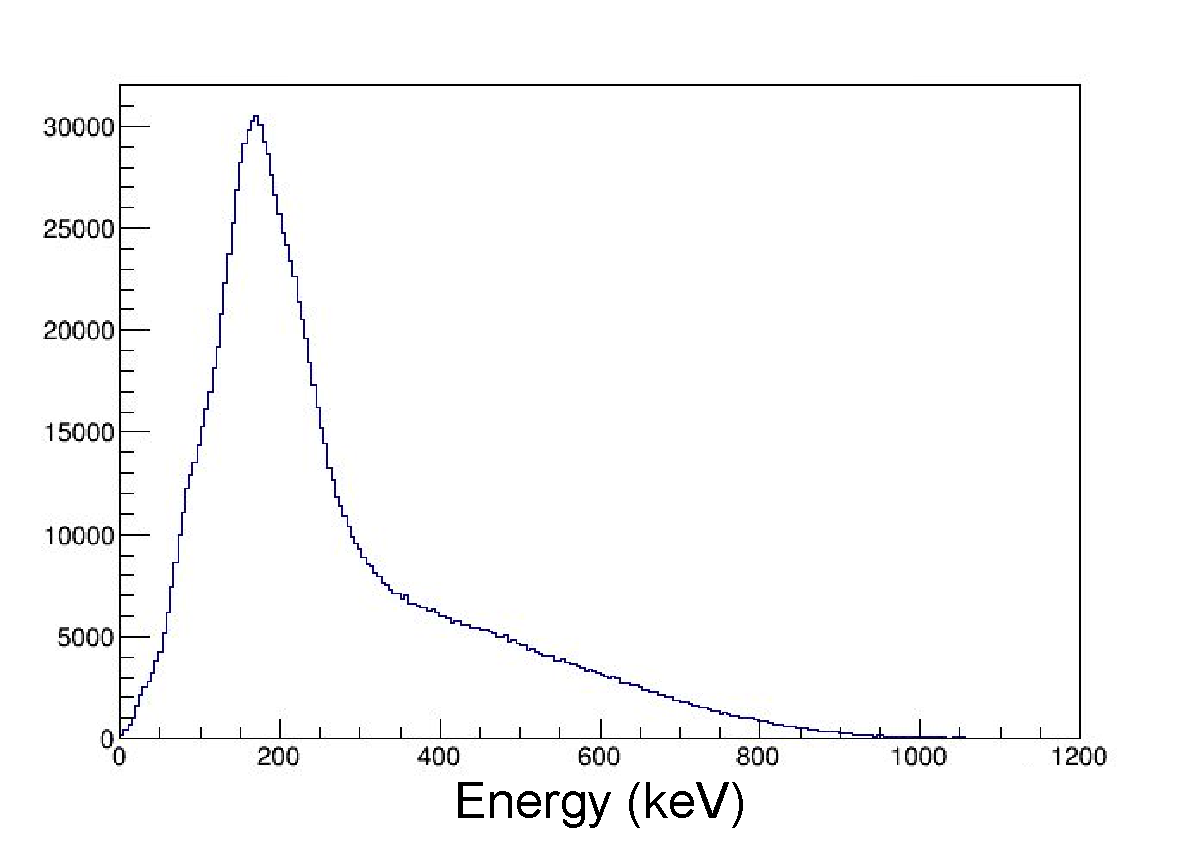
\includegraphics[scale=.5]{4-UCNACalibrations/xenonSpectrum.pdf}
\caption{Example energy spectrum of the neutron-activated xenon used for position map determination. }
\label{fig:xenonSpectrum}
\end{figure}

The spectral shape of the activated xenon changes with time due to the different half-lives
of the isotopes, but this is not a concern as the PMT will see the same shape at all positions
across the detector, just with different ADC scales due to the position dependence of the light
collection. Therefore one only needs to choose a feature of the spectrum to fit in different
positions to map the relative response.

\subsubsection{Position Maps}

The scintillator is divided into a grid of $5\times5\mathrm{~mm}^2$ squares (in the 1~T
decay trap coordinates) with one square directly in the center,
and the xenon events are collected for each of these ``pixels''. A key feature
from the spectrum is then chosen and fit in every pixel, with the position dependent response
factor in pixel $i$ for a single PMT defined as
%
\begin{equation}
  \eta_i = \frac{Q_i}{Q_0},
\end{equation}
%
where $Q_i$ is the fitted ADC value of the feature in pixel $i$ and $Q_0$ is the fitted ADC value of the
feature in the center pixel. This normalizes the position response for a PMT to the center pixel. The
position response at some position $(x,y)$, referred to as the continuous variable $\eta(x,y)$,
is then calculated via a two-dimensional Catmull-Rom
cubic interpolating spline \cite{catmull1974}. The same interpolation is used in the plots of the
position dependence in figure \ref{fig:posmaps}.


\begin{figure}[hp] 
\centering
\subfloat[East Detector]{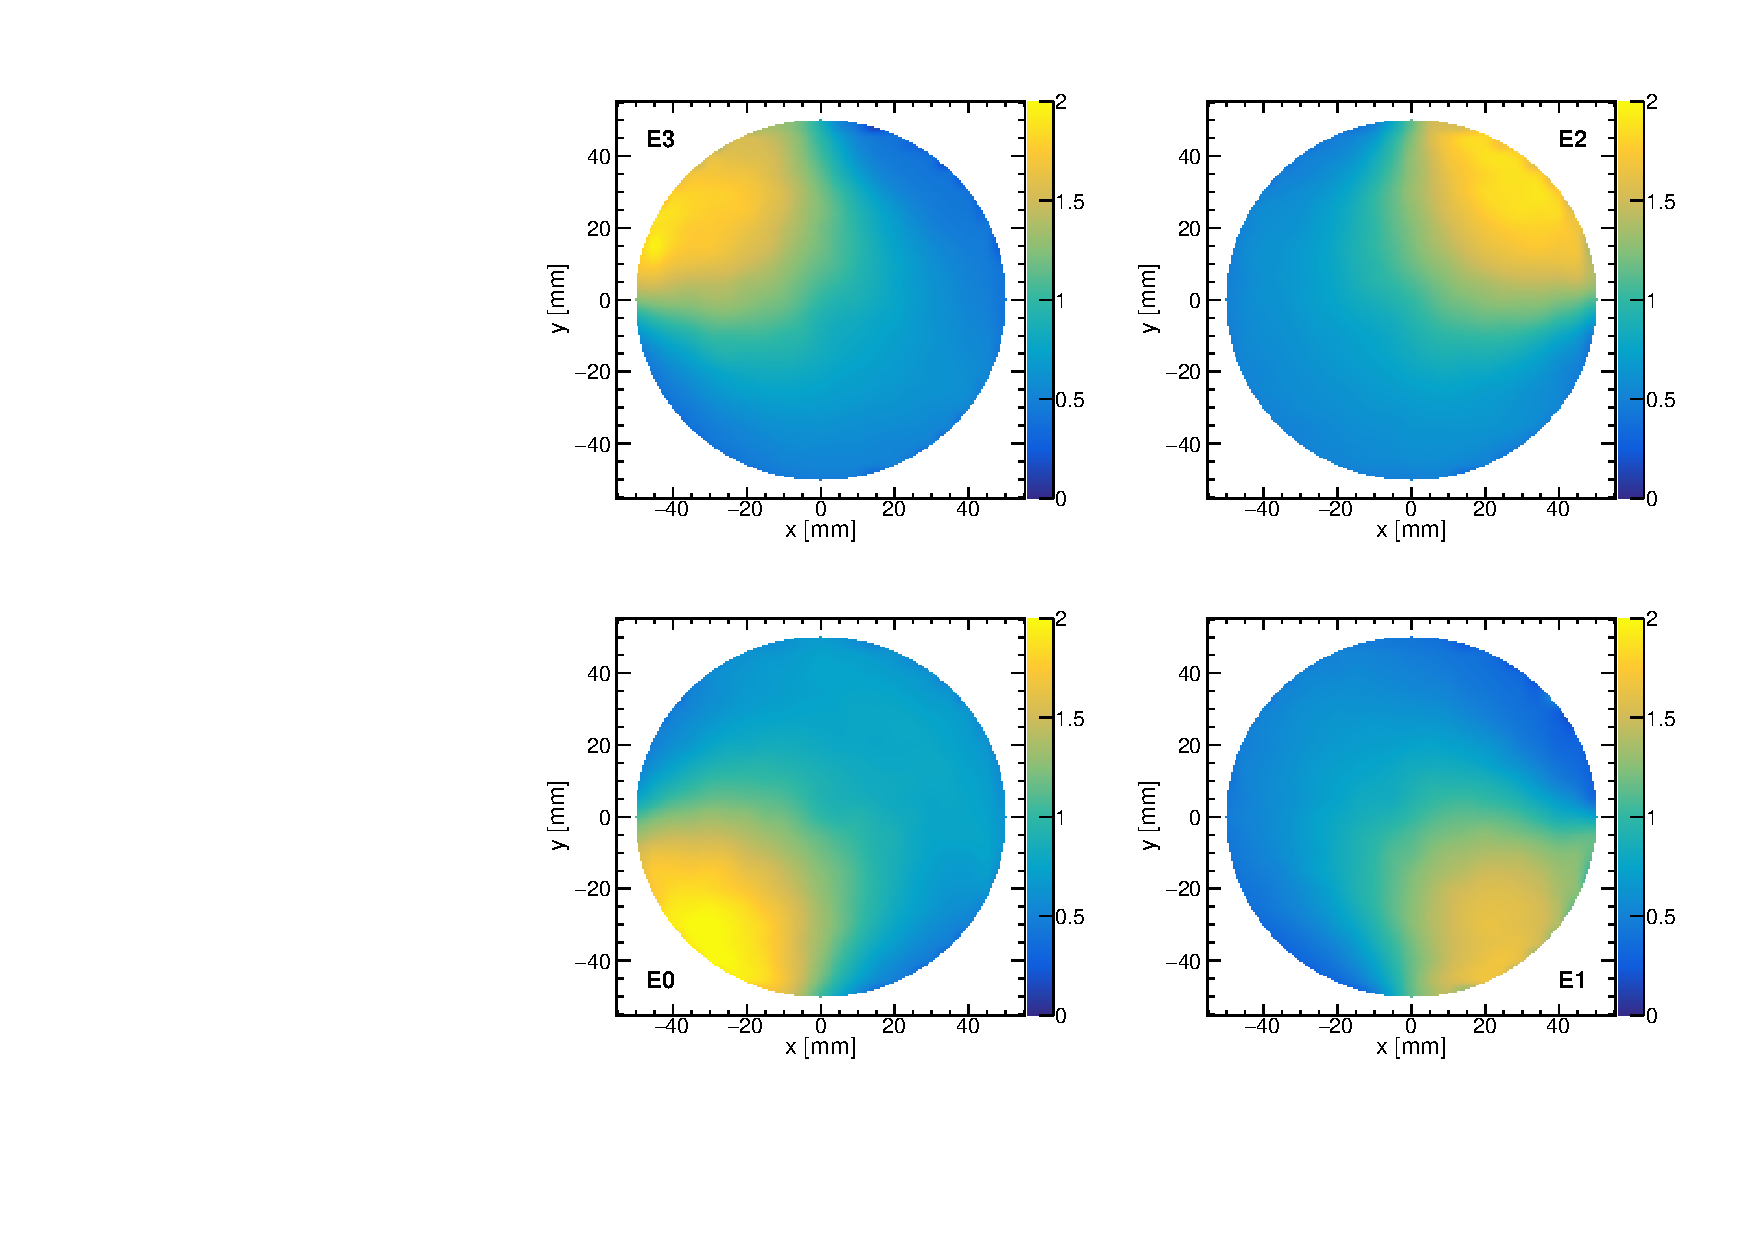
\includegraphics[page=1,scale=.55]{4-UCNACalibrations/position_map_4_5mm_endpoint.pdf}} \\
\subfloat[East Detector]{\includegraphics[page=2,scale=.55]{4-UCNACalibrations/position_map_4_5mm_endpoint.pdf}}
\caption{Typical set of position maps from a xenon position mapping period. The position maps
  remain fairly constant throughout the two run periods.}
\label{fig:posmaps}
\end{figure}

\begin{figure}[h] 
\centering
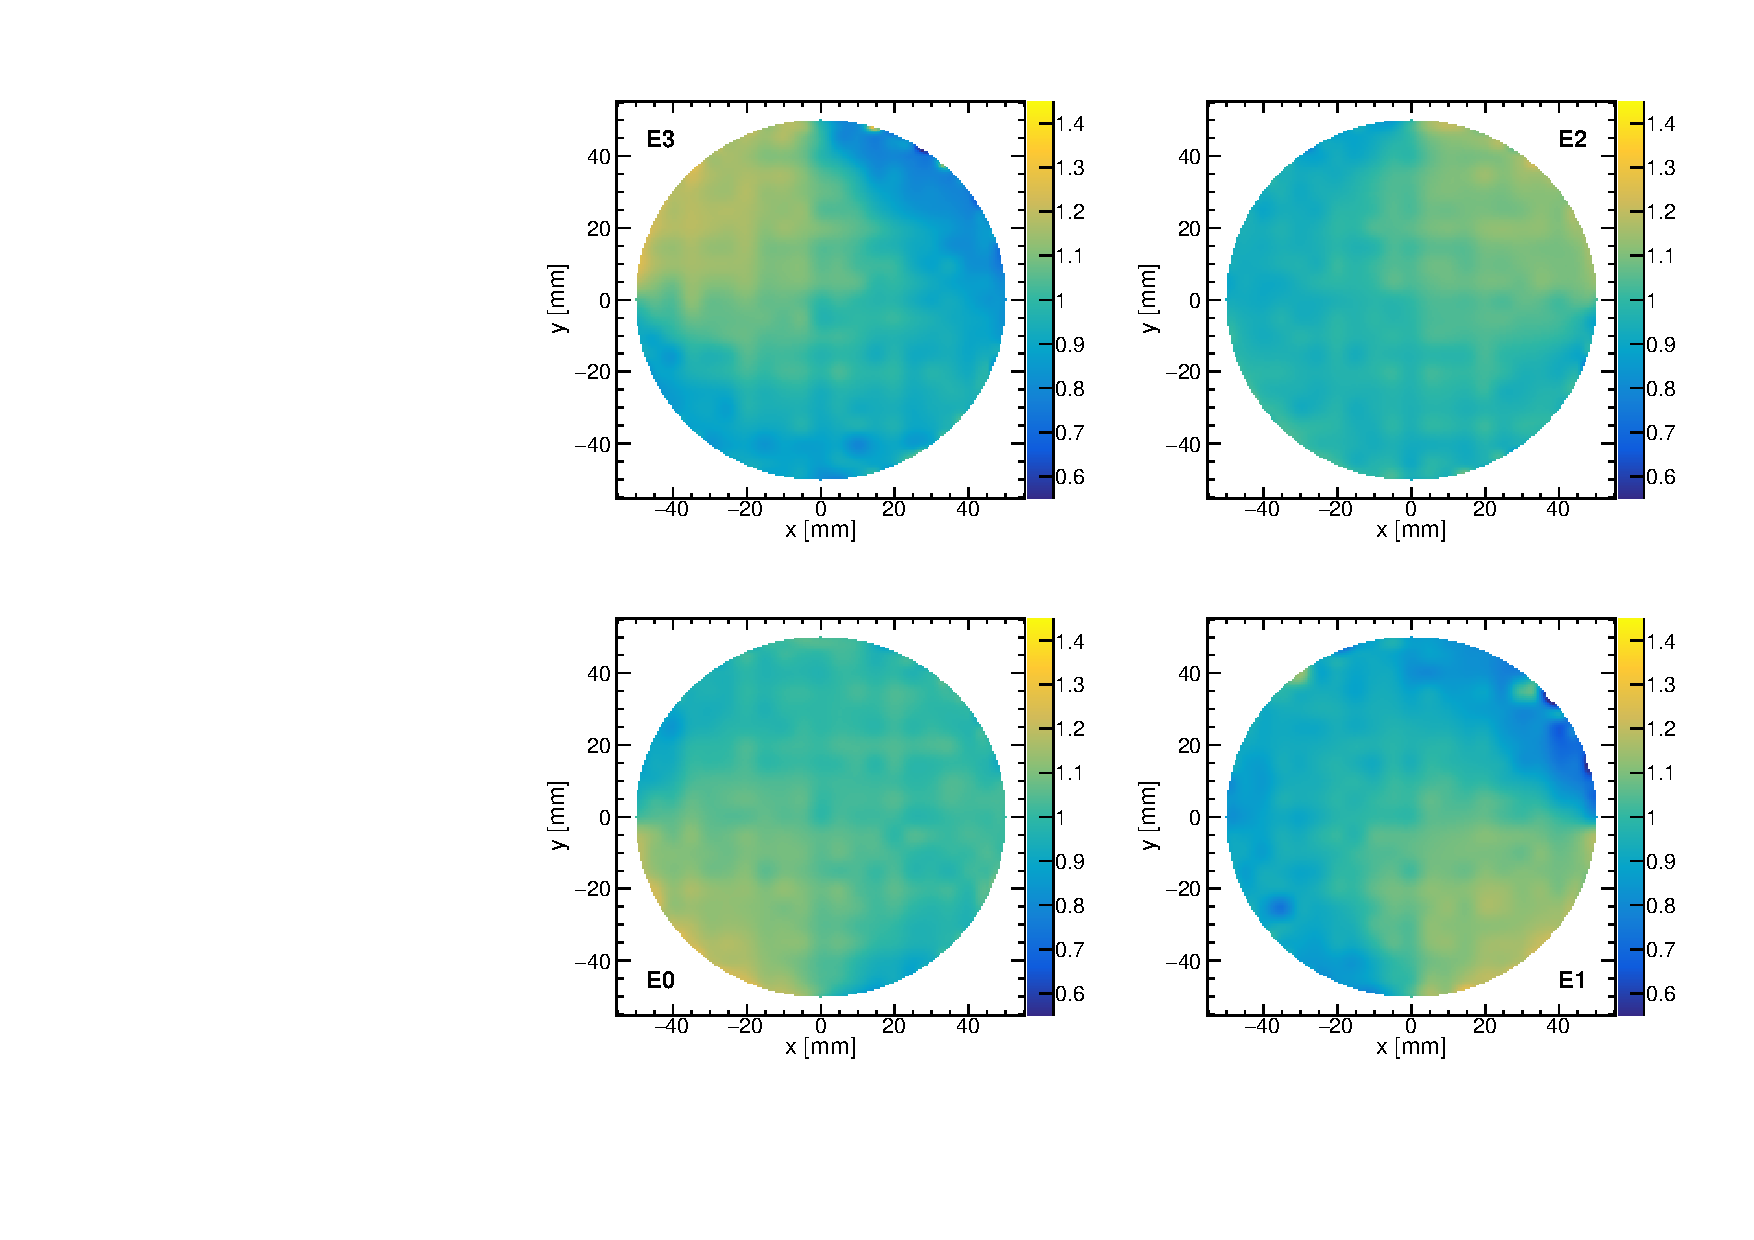
\includegraphics[scale=.55]{4-UCNACalibrations/posmapComp_4_5mm_endpoint_vs_peak.pdf}
\caption{Ratio of $\eta_{\mathrm{peak}} / \eta_{\mathrm{endpoint}}$ for the East side PMTs. The differences
  are most pronounced in areas of high and low light collection. The West side shows more
  consistency when comparing maps calculated using the different features.}
\label{fig:posmapCompare}
\end{figure}

A typical xenon energy spectrum can be seen in figure \ref{fig:xenonSpectrum}. The two obvious features one could
fit are the peak between 100~keV and 200~keV or the 915~keV $\beta$-decay endpoint. The peak is a
superposition of several isotopes, while the endpoint comes from the
$^{135}\mathrm{Xe~}\frac{3}{2}+$ isotope. The position maps are fit in terms of pedestal and gain corrected ADC,
so unfortunately the luxury of knowing an initial guess for the feature position is not afforded as it would
be if the fit was done in the energy domain. This makes
fitting the peak more reliable upon first inspection, as the endpoint fit (done via a Kurie plot as described
in section \ref{sssec:endpoint}) is more sensitive to the range of the fit especially when the spectrum is not
purely a $\beta$-spectrum. There is a problem with using the peak though, as areas with low light collection
for a given PMT lose a portion of the peak below the trigger threshold. This changes the feature shape
compared to regions of higher light output, thus biasing the position map. The better choice is then the
$^{135}\mathrm{Xe~}\frac{3}{2}+$ endpoint. 

The problem with fitting the endpoint in pixels with different light collection efficiencies is illustrated by
imagining that every pixel sees the same xenon energy spectrum (as in figure \ref{xenonSpectrum}), but that
the spectrum is compressed or stretched when compared to the spectrum in the center pixel depending on where
the pixel is located. Since each pixel has the same ADC range, choosing the proper fit range becomes difficult
as it is different in every pixel. To avoid this issue, a secondary feature was derived to be used as a
seed to the endpoint fit range. This secondary feature is calculated by first fitting the peak with a Gaussian
and extracting the mean ($\mu$) and sigma ($\sigma$), and then calculating the average ADC value, $\xi$, of the spectrum
from $\mu+1.5\sigma$ and beyond. Then the endpoint fit is done over the range $(\xi,2\xi)$. The range used to
calculate $\xi$ and the range over which the endpoint were fit were determined via trial and error, and produce
consistent results across the entire detector.

It should also be noted that the position maps were calculated using both the peak and the endpoint as the key
feature, and the differences are small. This is illustrated in figure \ref{fig:posmapCompare}, where the
ratio of the two methods is plotted.



\subsection{Wirechamber Energy Calibration}

\subsubsection{Method}

\subsubsection{Position dependence of anode signal}

\subsubsection{Relating Anode Signal to $E_{\mathrm{MWPC}}$}

\subsubsection{Backscattering Separation for Type 2/3 Events}
Should we put the 2/3 separation in the results chapter?

%----------------------------------------------------------

\section{Scintillator Energy Calibration}

\subsection{Method}
Talk about the parameters needed (resolution, trigger thresholds, pedestals, position maps, etc.)
Talk about the cyclical nature.
\subsection{Linearity Curves}
\subsection{PMT Resolution Factors} \label{ssec:PMTresolution}
\subsection{MC to Data Agreement}








